\documentclass{InsightArticle}

\usepackage[dvips]{graphicx}
\usepackage{float}
\usepackage{subfigure}

\usepackage[dvips,
bookmarks,
bookmarksopen,
backref,
colorlinks,linkcolor={blue},citecolor={blue},urlcolor={blue},
]{hyperref}

\title{Hough Transform Plane Detector}

% 
% NOTE: This is the last number of the "handle" URL that 
% The Insight Journal assigns to your paper as part of the
% submission process. Please replace the number "1338" with
% the actual handle number that you get assigned.
%
\newcommand{\IJhandlerIDnumber}{3250}

% Increment the release number whenever significant changes are made.
% The author and/or editor can define 'significant' however they like.
\release{0.00}

% At minimum, give your name and an email address.  You can include a
% snail-mail address if you like.

\author{Dorit Borrman and David Doria}
%\authoraddress{Rensselaer Polytechnic Institute, Troy NY \and Jacobs University}


\begin{document}

\IJhandlefooter{\IJhandlerIDnumber}


\ifpdf
\else
   %
   % Commands for including Graphics when using latex
   % 
   \DeclareGraphicsExtensions{.eps,.jpg,.gif,.tiff,.bmp,.png}
   \DeclareGraphicsRule{.jpg}{eps}{.jpg.bb}{`convert #1 eps:-}
   \DeclareGraphicsRule{.gif}{eps}{.gif.bb}{`convert #1 eps:-}
   \DeclareGraphicsRule{.tiff}{eps}{.tiff.bb}{`convert #1 eps:-}
   \DeclareGraphicsRule{.bmp}{eps}{.bmp.bb}{`convert #1 eps:-}
   \DeclareGraphicsRule{.png}{eps}{.png.bb}{`convert #1 eps:-}
\fi


\maketitle


\ifhtml
\chapter*{Front Matter\label{front}}
\fi

\begin{abstract}
\noindent
This document presents a wrapper of an extracted portion of 3DTK (http://threedtk.de) to enable a developer to find planes in 3D point cloud data.

The code is available here:
https://github.com/daviddoria/VTKHoughPlanes

\end{abstract}

\IJhandlenote{\IJhandlerIDnumber}

\tableofcontents
\section{Introduction}
Finding planes in 3D point clouds is a very common operation. This code uses the Hough transform to find the strongest planes in a point cloud and then labels each point with the label of the plane to which it belongs.

\section{Demonstration}
Figure \ref{fig:Demonstration} demonstrates the algorithm. Figure \ref{fig:Demonstration:InputPoints} shows a LiDAR scan of a flat panel monitor sitting on a counter. Figure \ref{fig:Demonstration:OutputPoints} shows the points colored by the plane to which they belong.

\begin{figure}[H]
\centering
\subfigure[Input points.]
  {
  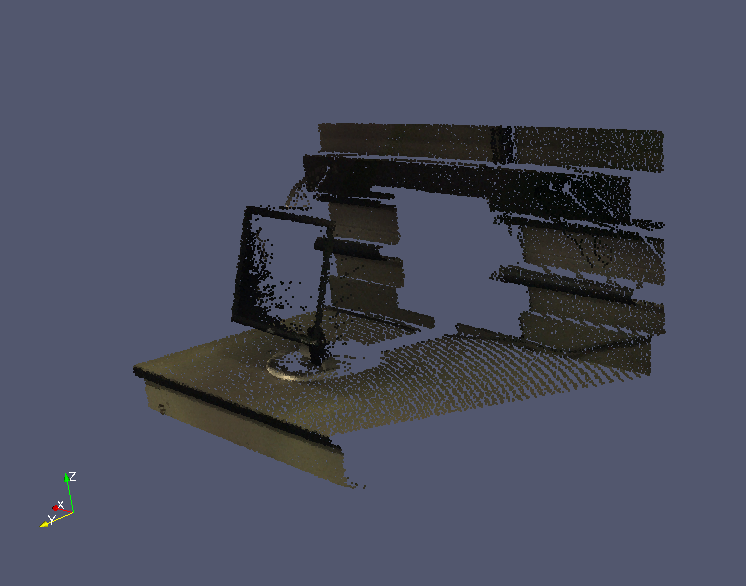
\includegraphics[width=0.3\linewidth]{images/counter}
  \label{fig:Demonstration:InputPoints}
  }
\subfigure[Output points.]
  {
  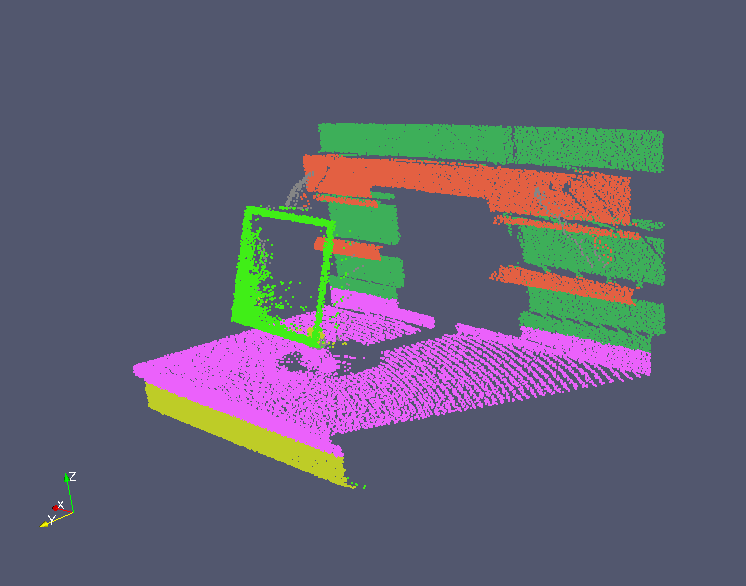
\includegraphics[width=0.3\linewidth]{images/counterPlanes}
  \label{fig:Demonstration:OutputPoints}
  }
\caption{Demonstration}
\label{fig:Demonstration}
\end{figure}

\subsubsection{Code Snippet}
The vtkHoughPlanes class must be passed an input vtkPolyData via SetInputConnection. The many parameters can also be set as demonstrated below.
\begin{verbatim}
  // Read the input file
  vtkSmartPointer<vtkXMLPolyDataReader> reader =
    vtkSmartPointer<vtkXMLPolyDataReader>::New();
  reader->SetFileName(inputFileName.c_str());
  reader->Update();
  
  vtkSmartPointer<vtkHoughPlanes> houghPlanes =
    vtkSmartPointer<vtkHoughPlanes>::New();
  houghPlanes->SetInputConnection(reader->GetOutputPort());
  houghPlanes->SetMaxDist(2.00);
  houghPlanes->SetMinDist(0.10);
  houghPlanes->SetAccumulatorMax(100);
  houghPlanes->SetMinSizeAllPoints(5);
  houghPlanes->SetRhoNum(100);
  houghPlanes->SetThetaNum(360);
  houghPlanes->SetPhiNum(176);
  houghPlanes->SetRhoMax(5.00);
  houghPlanes->SetMaxPointPlaneDist(0.050);
  houghPlanes->SetMaxPlanes(30);
  houghPlanes->SetMinPlaneSize(100);
  houghPlanes->SetMinPlanarity(0.300);
  houghPlanes->SetPlaneRatio(0.5);
  houghPlanes->SetPointDist(0.050);
  houghPlanes->SetPeakWindow(false);
  houghPlanes->SetWindowSize(8);
  houghPlanes->SetTrashMax(20);
  houghPlanes->SetAccumulatorType(1);
  houghPlanes->SetHoughAlgorithm(vtkHoughPlanes::Randomized);
  houghPlanes->Update();

  // Write output points colored by plane
  vtkSmartPointer<vtkXMLPolyDataWriter> writer = vtkSmartPointer<vtkXMLPolyDataWriter>::New();
  writer->SetInputConnection(houghPlanes->GetOutputPort());
  writer->SetFileName(outputFileName.c_str());
  writer->Write();

\end{verbatim}

%%%%%%%%%%%%%%%
% \begin{thebibliography}{9}
% 
% 	\bibitem{criminisi}
% 	  A. Criminisi, P. Perez, K. Toyama,
% 	  \emph{Object Removal by Exemplar-Based Inpainting}.
% 	  Computer Vision and Pattern Recognition 2003
% 
% \end{thebibliography}

\end{document}